%\section*{\giga{} indexing approach}
%\label{indexing}

\begin{figure*}[]   %%%%%%%%%%%%%%%%%%%%%%%
\centerline{
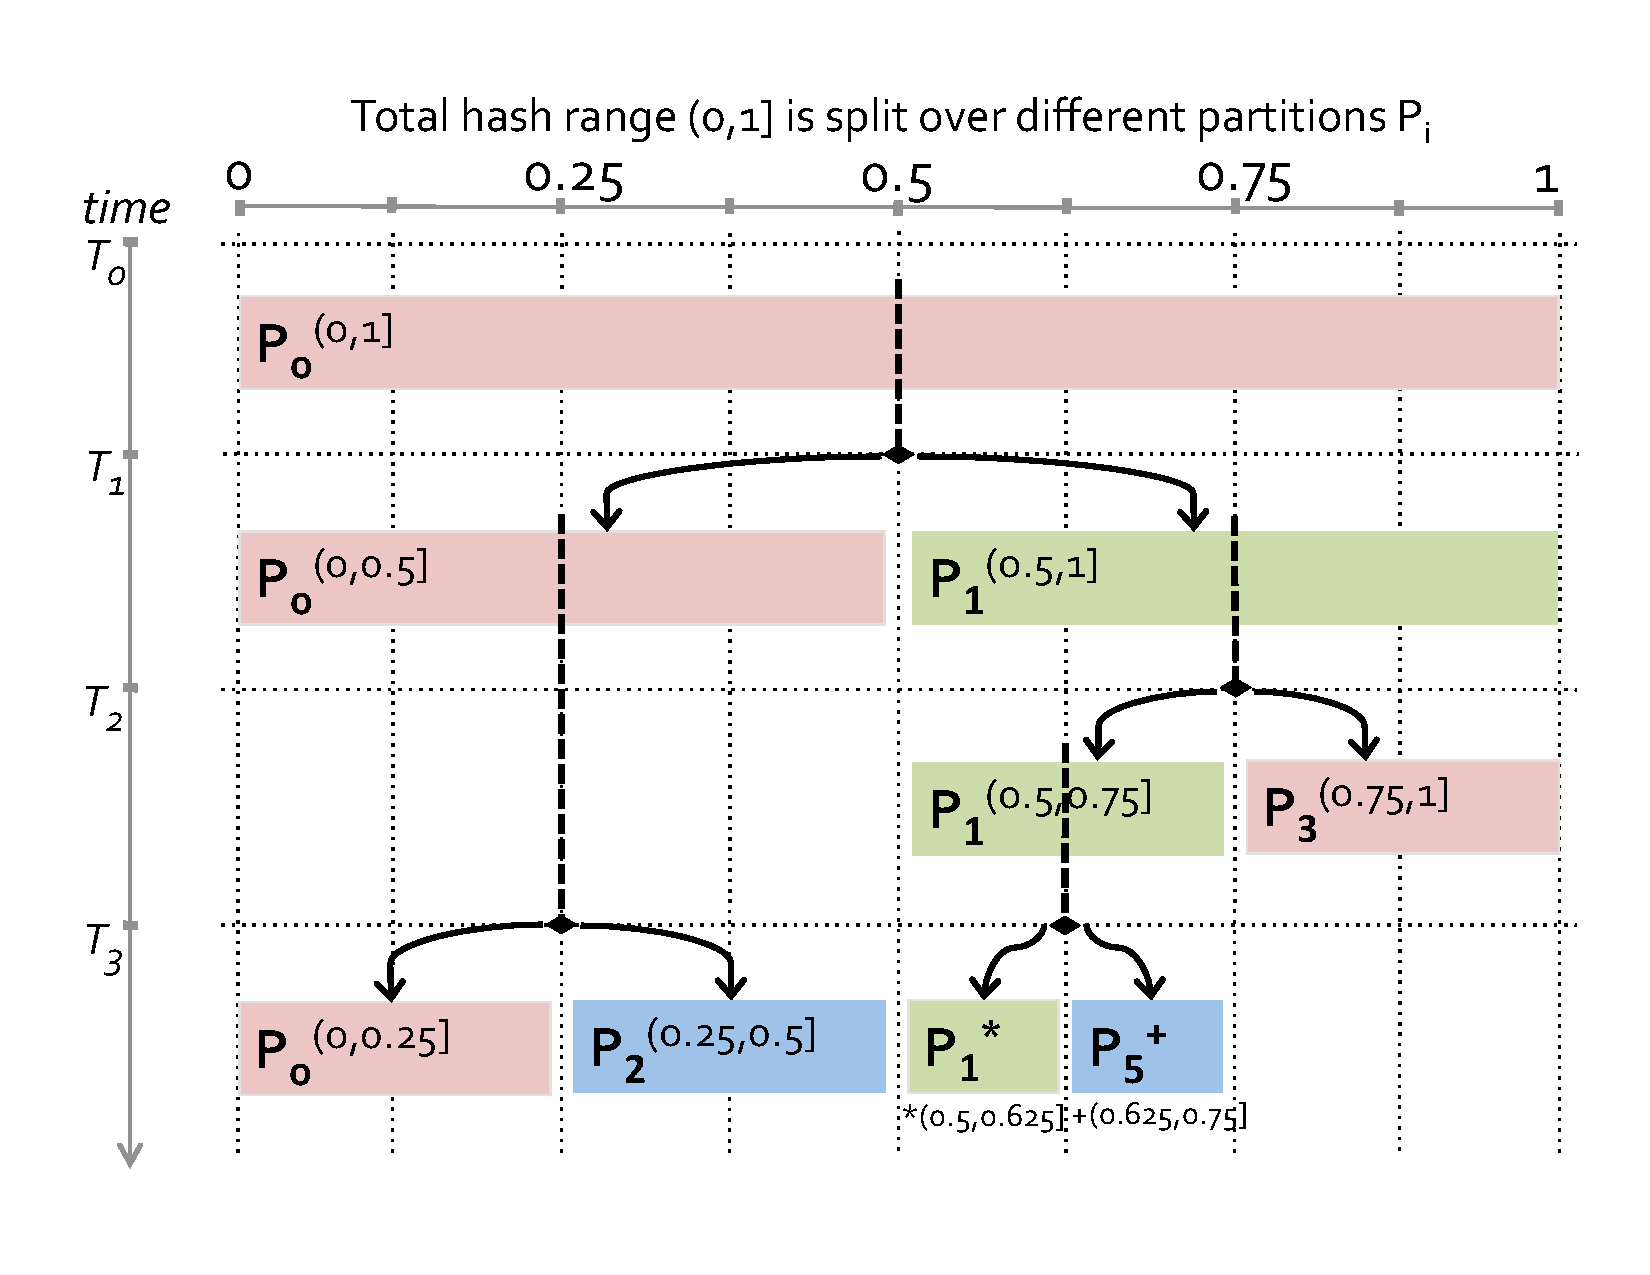
\includegraphics[scale=0.3]{figs/giga-partitioning-color}~~~
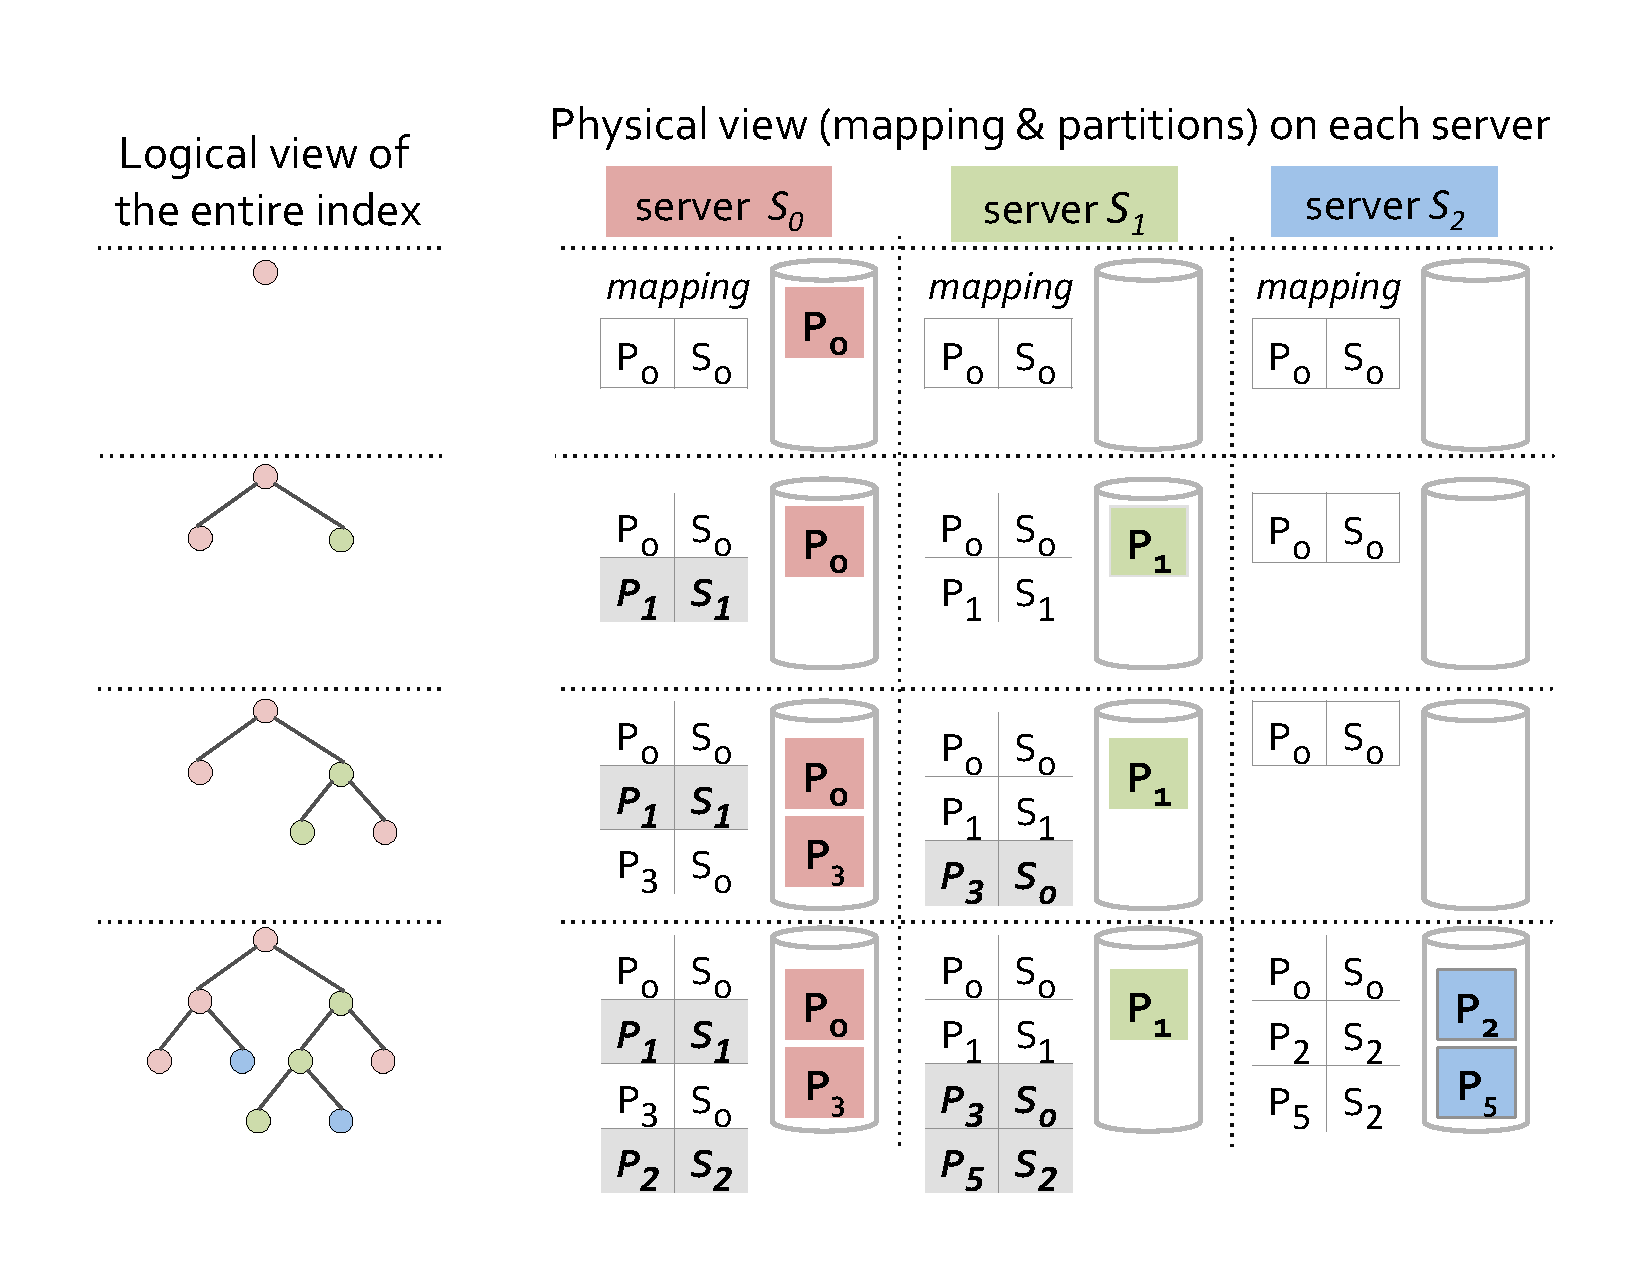
\includegraphics[scale=0.3]{figs/giga-mapping-color-new}
}
\vspace{-10pt}
\caption{\small 
\textbf{Concurrent and unsynchronized data partitioning in \giga{}.}
The hash-space $(0,1]$ is divided into multiple partitions ($P_i$) that
are distributed over many servers (different colors).
An index starts small (on one server) and scales out incrementally by 
enabling each server to independently split its partitions \textit{without
global co-ordination}.
Each server has a \textit{local, partial view} of the entire index which
includes the partitions they store and the history of splits of these
partitions (shaded entry in the mapping table).
}
%\vspace{10pt}
%\hrule depth 0.5pt
\label{fig:giga-indexing}
\end{figure*}    %%%%%%%%%%%%%%%%%%%%%%%

\giga{} uses a combination of three ideas to push the limits of 
scalability and concurrency of file system directories: 
scale-out data partitioning on servers without any system-wide synchronization, 
allowing the use of out-of-date partition-to-server mapping state, and 
facilitating online server addition with minimal data migration overhead
\citep{GIGA}.
We discuss the first two ideas in details

\textbf{Unsynchronized data partitioning -- }
%\subsection*{Unsynchronized data partitioning}
%\label{indexing:partitioning}
\giga{} uses hash-based indexing to incrementally divide each directory into
multiple partitions that are distributed over multiple servers.
Each filename (contained in a directory entry) is hashed and then mapped to a 
partition using an index. 
Our implementation uses the cryptographic MD5 hash but is not specific
to it.
\giga{} relies only on one property of the selected function: for any 
distribution of unique filenames, the hash values of these filenames must 
be uniformly distributed in the hash space \citep{md5:rfc1321}.

Figure \ref{fig:giga-indexing} shows how \giga{} indexing grows incrementally.
In this example, a directory is to be spread over three servers 
$\{S_0, S_1, S_2\}$ in three colors.
$P_i^{(x,y]}$ denotes the hash-space range $(x,y]$ held by a partition with the
unique identifier $i$.
%\footnote{For simplicity, we disallow the hash value 
%zero from being used.}
\giga{} uses the identifier $i$ to map $P_i$ to an appropriate server $S_i$
using a round-robin mapping, 
i.e., server $S_i$ is $i$~\texttt{\small{modulo}}~$num\_servers$.
%(Section \ref{indexing.reconfig} addresses growing the number of servers)
The color of each partition indicates the (color of the) server it resides on. 
Initially, at time $T_0$, the directory is small and stored on a single 
partition $P_0^{(0,1]}$ on server $S_0$.
As the directory grows and the partition size exceeds a threshold number of
directory entries, 
provided this server knows of an underutilized server, 
$S_0$ splits $P_0^{(0,1]}$ into two by moving the greater half of its
hash-space range to a new partition $P_1^{(0.5,1]}$ on $S_1$.
As the directory expands, servers continue to split partitions onto 
more servers until all have about the same fraction of the hash-space
to manage. 
\giga{} computes a split's target partition identifier using well-known 
radix-based techniques.
%\footnote{
%\giga{} calculates the identifier of partition $i$ using the depth of the tree,
%$r$, which is derived from the number of splits of the zeroth partition $P_0$.
%Specifically, if a partition has an identifier $i$ and is at tree depth $r$, 
%then in the next split $P_i$ will move half of its filenames, from the  
%larger half of its hash-range, to a new partition with identifier $i+2^r$.
%After a split completes, both partitions will be at depth $r+1$ in the tree.
%In Figure \ref{fig:giga-indexing}, for example, partition $P_1^{(0.5,0.75]}$,
%with identifier $i = 1$, is at tree depth $r = 2$.
%A split causes $P_1$ to move the larger half of its hash-space $(0.625,0.75]$ 
%to the newly created partition $P_5$, and both partitions are then at tree 
%depth of $r$ = 3.
%}

The key goal for \giga{} is for each server to split independently,
without system-wide serialization or synchronization.
Accordingly, servers make local decisions to split a partition. 
The side-effect of uncoordinated growth is that \giga{} servers do not have 
a global view of the partition-to-server mapping on any one server; each server 
only has a partial view of the entire index (the mapping tables in Figure 
\ref{fig:giga-indexing}).
Other than the partitions that a server manages, a server knows only the
identity of the server that knows more about each ``child'' partition resulting
from a prior split by this server.
In Figure \ref{fig:giga-indexing}, at time $T_3$, server $S_1$ manages partition
$P_1$ at tree depth $r = 3$, and knows that it previously split $P_1$ to create 
children partitions, $P_3$ and $P_5$, on servers $S_0$ and $S_2$ respectively.
Servers are mostly unaware about partition splits that happen 
on other servers (and did not target them); for instance, at time $T_3$, 
server $S_0$ is unaware of 
partition $P_5$ and server $S_1$ is unaware of partition $P_2$.

Specifically, each server knows only the split history of its partitions.
The full \giga{} index is a complete history of the directory partitioning, 
which is the transitive closure over the local mappings on each server.
This full index is also not maintained synchronously by any client.
\giga{} clients can enumerate the partitions of a directory by traversing 
its split histories starting with the zeroth partition $P_0$.
However, such a full index constructed and cached by a client may be stale at
any time, particularly for rapidly mutating directories.
%\footnote{
%In the file system world, this is analogous to enumeration of all file system
%blocks done by the consistency checker (\texttt{fsck}) which starts at the 
%superblock and traverses the blocks of all files by following the direct-, 
%indirect- and doubly indirect-pointers of the file's i-node.
%}
%This transitivity enabled by split histories is useful for two reasons.
%First, split histories can help recreate the data-structures used to maintain
%the \giga{} index.
%For instance, lost or corrupted mapping information can be reconstructed by 
%traversing the split histories of a partition to learn about other partitions
%and their servers.
%And second, split histories enables \giga{} to tolerate inconsistent, out-of-date
%mapping state at the clients (described later in Section 
%\ref{indexing:inconsistency}).
%Split histories enable \giga{} servers to correct inconsistent, out-of-date
%mapping state at the clients.

%XXX:optimizations:
%- splitting over all servers once is enough, but load imbalance
%- split into half -> split into N over N servers: adaptive fast growth

%%%%%%%%%%%
\textbf{Tolerating inconsistent mapping at clients -- }
%\subsection*{Tolerating inconsistent mapping at clients}
%\label{indexing:inconsistency}
Clients seeking a specific filename find the appropriate partition by probing 
servers, possibly incorrectly, based on their cached index.
To construct this index, a client must have resolved the directory's parent
directory entry which contains a cluster-wide i-node identifying the server and
partition for the zeroth partition $P_0$.
Partition $P_0$ may be the appropriate partition for the sought filename, or it
may not because of a previous partition split that the client has not yet
learned about. 
An ``incorrectly'' addressed server detects the addressing error by recomputing 
the partition identifier by re-hashing the filename.
If this hashed filename does not belong in the partition it has,
this server sends a split history update to the client.
The client updates its cached version of the global index and 
retries the original request.

The drawback of allowing inconsistent indices is that clients may need 
additional probes before addressing requests to the correct server.
The required number of incorrect probes depends on the client request 
rate and the directory mutation rate (rate of splitting partitions).
It is conceivable that a client with an empty index may send O$(log(N_p))$ 
incorrect probes, where $N_p$ is the 
number of partitions, but \giga{}'s split history updates makes this many
incorrect probes unlikely.
Each update sends the split histories of all partitions that reside on a
given server, filling all gaps in the client index known to this server and
causing client indices to catch up quickly.
Moreover, after a directory stops splitting partitions, clients soon after will 
no longer incur any addressing errors.
%\giga{}'s eventual consistency for cached indices is different from LH*'s
%eventual consistency because the latter's idea of independent splitting (called
%pre-splitting) suffers addressing errors even when the index
%stops mutating \citep{lh*:litwin96}. 

\textbf{Key performance insights -- }
Detailed analysis of the scalability and performance of \giga{} studies several
tradeoffs \citep{giga}; the observations that are within the scope of this work
include the load-balancing and incremental growth strategy.


\begin{comment}
%%%%%%%%%%%
\subsection*{On-line server additions}
\label{indexing.reconfig}

%This section describes how \giga{} adapts to the addition of servers in a 
%running directory service.
%\footnote{Server removal (i.e., decommissioned, not 
%failed and later replaced) is not as
%important for high performance systems so we leave it to be done by user-level
%data copy tools.}

\begin{figure}[t]
\centerline{\includegraphics[scale=0.35]{../common/figures/giga-serveradd}}
\vspace{-10pt}
\caption{\small
\textbf{\giga{} server additions.}
By changing the partition-to-server mapping from round-robin on the original 
server set to sequential on the newly added servers, \giga{} can minimize the amount
of data migrated (shown by arrows indicating splits).
}
\label{fig:giga-adding}
%\vspace{10pt}
%\hrule depth 0.5pt
\end{figure}

When new servers are added to an existing configuration, the system is
immediately no longer load balanced, and it 
should re-balance itself by migrating a minimal number of directory entries
from all existing servers equally. 
Using the round-robin partition-to-server mapping, shown in Figure 
\ref{fig:giga-indexing}, a naive server addition scheme would require 
re-mapping almost all directory entries whenever a new server is added.

\giga{} avoids re-mapping all directory entries on addition of servers by 
differentiating
the partition-to-server mapping for initial directory growth from the mapping
for additional servers.
For additional servers, \giga{} does not use the round-robin partition-to-server
map (shown in Figure \ref{fig:giga-indexing}) and instead 
maps all future partitions to the new servers in a ``sequential manner''.
The benefit of round-robin mapping is faster exploitation of parallelism
when a directory is small and growing, while a sequential mapping for the tail
set of partitions does not disturb previously mapped partitions more than is 
mandatory for load balancing.
Figure \ref{fig:giga-adding} shows an example where the original configuration
has 5 servers with 3 partitions each, and partitions $P_0$ to $P_{14}$ use a 
round-robin rule (for $P_i$, server is $i$ \texttt{mod} $N$, where $N$ is 
number of servers).
After the addition of two servers, the six new partitions $P_{15}$-$P_{20}$
will be mapped to servers using the new mapping rule: $i$ \texttt{div} $M$, 
where $M$ is the number of partitions per server (e.g., 3 partitions/server).

In \giga{} even the number of servers can be stale at servers and clients. 
The arrival of a new server and its order in the global server list is declared
by the cluster file system's configuration management protocol, such as
Zookeeper for HDFS \citep{zookeeper:hunt10}, leading to each existing server
eventually noticing the new server.
Once it knows about new servers, an existing server can inspect its partitions
for those that have sufficient directory entries to warrant splitting and would
split to a newly added server.
The normal \giga{} splitting mechanism kicks in to migrate only directory
entries that belong on the new servers.
The order in which an existing server inspects partitions can be entirely
driven by client references to partitions, biasing migration in favor of active
directories.
Or based on an administrator control, it can also be driven by a background 
traversal of a list of partitions whose size exceeds the splitting threshold. 

\end{comment}
